\chapter{Newton-Verfahren}
\lhead{Newton-Verfahren}
\rhead{}

\section{Nullstellen von Funktionen}
\rhead{Nullstellen von Funktionen}
\begin{figure}
\centering
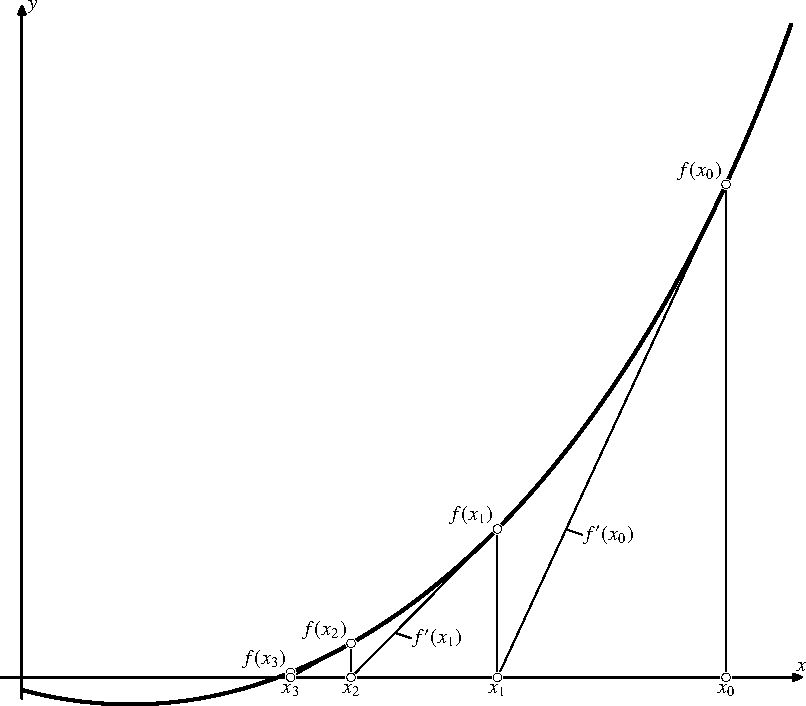
\includegraphics{chapters/images/randwert-2.pdf}
\caption{Bestimmung der Nullstelle einer Funktion $f(x)$ mit dem
Newton-Verfahren.
Die Approximation $x_{n+1}$ wird gefunden als Schnittpunkt der Tangente
im Punkt $(x_n,f(x_n))$ (mit Steigung $f'(x_n)$) mit der $x$-Achse.
\label{newton:graphik}}
\end{figure}
Das Ziel dieses Anhangs ist, die folgende Aufgabe numerisch zu l"osen:
\begin{aufgabe}
Gegen ist eine differenzierbar Funktion
$f\colon\mathbb R\to\mathbb R:x\mapsto f(x)$
und eine Zahl $y$ im Wertebereich von $f$.
Finde $\hat{x}\in\mathbb R$ so, dass $f(\hat{x})=y$.
\end{aufgabe}
Im allgemeinen kann man nicht davon ausgehen, dass sich eine L"osung der
Gleichung $f(x)=y$ in geschlossener Form finden l"asst.
Nur einige wenige Klassen von Gleichungen haben L"osungsformeln dieser Art.
Wir beschr"anken uns daher auf das Problem, eine Approximation f"ur die
L"osung zu bestimmen.

Indem wir statt der Funktion $f(x)$ die Funktion $x\mapsto g(x)=f(x)-y$
betrachten, k"onnen wir die gesuchte Zahl $x$ auch als L"osung der
Gleichung $g(x)=0$ finden:
\begin{equation}
f(x)=y
\qquad\qquad
\Rightarrow
\qquad\qquad
g(x)=f(x)-y = 0.
\label{newton:reduktion}
\end{equation}
Es gen"ugt also, ein L"osungsverfahren zu entwickeln f"ur die Aufgabe
\begin{aufgabe}
Gegen ist eine differenzierbar Funktion
$f\colon\mathbb R\to\mathbb R:x\mapsto f(x)$,
finde $\hat{x}\in\mathbb R$ so, dass $f(\hat{x})=0$.
\end{aufgabe}
Da wir nur eine numerische L"osung brauchen, versuchen wir sie dadurch
zu finden, dass wir eine Anfangssch"atzung $x_0$ wiederholt korrigieren,
bis der Fehler klein genug ist.
Es soll also eine Folge $x_0,x_1,x_2,\dots$ konstruiert werden, welche
gegen die L"osung $\hat{x}$ konvergiert.
Der Differenzenquotient ist eine Approximation f"ur die Steigung
$f'(x_n)$,
\begin{equation}
\frac{
f(x_{\mathstrut n+1})-f(x_{\mathstrut n})
}{
x_{\mathstrut n+1}-x_{\mathstrut n}
}
\simeq = f'(x_n).
\label{newton:pre}
\end{equation}
Wir m"ochten gerne, dass $f(x_{n+1})=0$ ist, und k"onnen (\ref{newton:pre})
unter dieser Annahme nach $x_{n+1}$ aufl"osen:
\begin{align*}
-f(x_n)
&\simeq
f'(x_n)\,(x_{\mathstrut n+1}-x_{\mathstrut n})
\\
x_{\mathstrut n}-\frac{f(x_n)}{f'(x_n)}
&\simeq x_{\mathstrut n+1}
\end{align*}
Damit haben wir ein L"osungsverfahren gefunden:
\begin{satz}[Newton]
Ist $f$ eine differenzierbare Funktion, deren Ableitung bei der Nullstelle
$\hat{x}$ nicht verschwindet, also $f(\hat{x})\ne 0$, und $x_0$ eine erste
Approximation f"ur $\hat{x}$, dann konvergiert die Folge
definiert durch die Rekursionsformel
\[
x_{n+1}=x_n-\frac{f(x_n)}{f'(x_n)},
\]
dann konvergiert $x_n$ gegen $\hat{x}$, falls $x_0$ nahe genug bei
$\hat{x}$ liegt.
\end{satz}

\begin{beispiel}
Man finde die Wurzel der Zahl $y$, d.~h.~man muss die Nullstellen
der Funktion $f(x)=x^2-y$ finden.
Das Newton-Verfahren ben"otigt die Ableitung von $f$, sie ist
$f'(x)=2x$, und konstruiert daraus die Folge
\begin{equation}
x_{n+1} = x_n - \frac{f(x_n)}{f'(x_n)}=x_n-\frac{x_n^2-y}{2x_n}
=
\frac{2x_n^2-x_n^2+y}{2x_n}
=
\frac12\biggl(x_n + \frac{y}{x_n}\biggr)
\label{newton:mittel}
\end{equation}
Die Quaratwurzel von $y$ erf"ullt nat"urlich
\[
\sqrt{y} = \frac12\biggl( \sqrt{y}+\frac{y}{\sqrt{y}}\biggr).
\]
Mit $x_n$ ist auch $y/x_n$ eine Approximation von $\sqrt{y}$.
Die neue Approximation $x_{n+1}$ ist das arithmetische Mittel der
beiden Approximationen $x_n$ und $y/x_n$ von $\sqrt{y}$.
Die Konvergenz dieser Folge ist sehr schnell, wie Tabelle~\ref{newton:sqrt2}
zeigt.
\begin{table}
\centering
\begin{tabular}{|>{$}r<{$}|>{$}r<{$}|}
\hline
n&x_n\\
\hline
0 &  2.00000000000000\\
1 &  1.50000000000000\\
2 &  1.\underline{41}666666666667\\
3 &  1.\underline{41421}568627451\\
4 &  1.\underline{41421356237}469\\
5 &  1.\underline{41421356237309}\\
6 &  1.\underline{41421356237309}\\
\hline
\end{tabular}
\caption{Approxmationen von $\sqrt{2}$ mit Hilfe des Newton-Algorithmus,
korrekte Stellen unterstrichen.
Die Anzahl korrekter Stellen verdoppelt sich in jedem Schritt.
\label{newton:sqrt2}}
\end{table}
In jedem Schritt verdoppelt sich die Anzahl korrekter Stellen.
Dies ist eine allgemeine Eigenschaft des Newton-Algorithmus, wie
in Abschnitt~\ref{section:newton:konvergenz} erkl"art wird.
\end{beispiel}

\section{Konvergenzgeschwindigkeit\label{section:newton:konvergenz}}

\section{L"osung von Vektorgleichungen\label{section:newton:vektor}}
\rhead{L"osung von Vektorgleichungen}
Wir m"ochten das Verfahren nun erweitern, so dass wir nicht nur eine
einzige Gleichung $f(x)=y$ nach $x$ aufl"osen k"onnen, wir m"ochten dazu 
f"ur ein Gleichungssystem von nichtlinearen Gleichungen
\begin{align*}
f_1(x_1,\dots,x_n)&=y_1\\
f_2(x_1,\dots,x_n)&=y_2\\
&\;\;\vdots\\
f_m(x_1,\dots,x_n)&=y_m
\end{align*}
ebenfalls in der Lage sein.
Wie bei einer einzigen Gleichung k"onnen wir das Problem reduzieren
auf das Finden von gleichzeitigen Nullstellen der Funktionen $g_i$ mit
\begin{align*}
g_1(x_1,\dots,x_n)&=f_1(x_1,\dots,x_n)-y_1=0\\
g_2(x_1,\dots,x_n)&=f_2(x_1,\dots,x_n)-y_2=0\\
&\;\;\vdots\\
g_m(x_1,\dots,x_n)&=f_m(x_1,\dots,x_n)-y_m=0.
\end{align*}









